\documentclass[10pt]{article}

\usepackage{mi_lab_include_2015-06-01}


\rhead{{\color{HeadingColor}VP04 Gravitational Force}}


\begin{document} 

\begin{center}
{\color{HeadingColor}{{\LARGE {\textbf{Calculating and Visualizing Gravitational Force}}}}}
\end{center}

\section*{Objectives}

In order to model the motion of gravitationally interacting bodies, it is necessary to be able to instruct a computer to calculate a gravitational force and to display an arrow representing the force. Before doing this activity you should have read Section 3.6 of the \MI textbook, which discusses the structure of a computational model that includes the gravitational force.\\

After completing this activity you should be able to:\\

\begin{compactitem}[\color{MIBlue}$\bullet$]
\item Write a VPython program to calculate a gravitational force
\item To create and scale an \code{arrow} to represent a vector quantity such as a force on an object
\item To write a \while loop that creates multiple objects and performs the same calculation on each one\\
\end{compactitem}

\section{Prediction}

\begin{compactitem}[\color{MIRed}$\Rightarrow$]
\item On a whiteboard draw a diagram like the one below.  Each numbered dot represents the position of a different spacecraft. (A single spacecraft near a planet would not move in a straight line.)
\item At each numbered location draw an arrow representing the gravitational force on a spacecraft at that location, due to the planet.
\item Make sure that your diagram makes sense.  Is the direction of each arrow correct? Is the length of the arrow proportional to the magnitude of the quantity it represents?\\
\end{compactitem}

\begin{center}
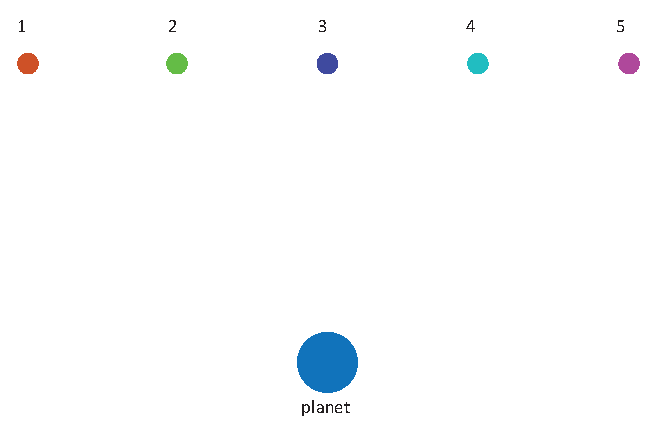
\includegraphics{planet_5_spacecraft.eps}
\end{center}

\vspace*{10pt}
\checkpoint

\section{Objects and Constants}

\subsection{Creating Objects}

\begin{compactitem}[\color{MIRed}$\Rightarrow$]
\item Start a VPython program by inserting these lines at the beginning:\\
\color{CodeColor}
\begin{verbatim}
from __future__ import division, print_function
from visual import *
scene.width = 1000
\end{verbatim}
\color{black}
\vspace*{10pt}
\item Create a sphere of radius \po{6.4}{6} m, located at \mivec{0,\po{-2}{7},0} m to represent the planet. Give the sphere an appropriate name.
\item Create a second sphere to represent the spacecraft. Give this sphere an appropriate name. You will need to exaggerate its radius to make it visible; try \po{3}{6} m.  Place it at location \mivec{\po{-13}{7},\po{4.5}{7},0} m, and make its color different from the color of the planet.
\end{compactitem}

\subsection{Constants}

In a program it is important to use symbolic names for constants.  Why?  To make it easy to make changes and corrections to the model.  For example, if you want to change the mass of an object, it is much easier to change a single line such as :

\color{CodeColor}
\begin{verbatim}
mass = 1.3e7
\end{verbatim}
\color{black}

than it is to search for and replace all occurrences of the string \color{CodeColor}\texttt{1.3e7}\color{black}.\\

\begin{compactitem}[\color{MIRed}$\Rightarrow$]
\item Insert a line of code that assigns the name ``G'' to the value of the gravitational constant.
\item Also create approriately named variables to store the masses of the planet (\po{6}{24} kg) and of a spacecraft (\po{1.5}{4} kg).\\
\end{compactitem}

\section{Calculating Gravitational Force}

For the single spacecraft your program has created:\\
\begin{compactitem}[\color{MIRed}$\Rightarrow$]
\item Add instructions to calculate gravitational force on the spacecraft by the planet. Use symbolic names for every quantity in the program lines you write.
\item Print the value you calculated.  Does the direction of the force make sense?
\end{compactitem}

\subsection{Representing Gravitational Force with an Arrow}  

\begin{compactitem}[\color{MIRed}$\Rightarrow$]
\item Create an \code{arrow} object with its tail at the location of the spacecraft.  
\item Set the \code{axis} of the \code{arrow} object to the value of the gravitational force you calculated.
\item Run the program.  What do you see?  Can you explain why?
\end{compactitem}

\subsection{Scale Factors}

We will frequently want to use \code{arrow} objects to visualize vector quantities such as forces.  However, if the distances between objects in the program is very large compared to the magnitude of the vector, the \code{arrow} may be too small to see.  (Alternatively, if the distance between objects is very small compared to the magnitude of the vector, the \code{arrow} object may be so huge that no other objects can be seen.)\\

\begin{compactitem}[\color{MIRed}$\Rightarrow$]
\item Watch the VPython instructional video \textit{VPython Instructional Videos: 5. Scale Factors }\\ \url{http://vpython.org/video05.html} to see how to multiply the \code{axis} attribute of an \code{arrow} by a scalar to adjust its length so all objects in the scene are visible.
\item Use an appropriate scale factor to scale your \code{arrow} to an appropriate length.  Be prepared to explain how you determined this scale factor.\\
\end{compactitem}

\checkpoint

\section{Multiple Locations}

To calculate and display the gravitational force on several spacecraft at different locations, as in the diagram you drew previously, we can use a loop.  Recall that in a previous activity you encountered two different kinds of loops:  one that created multiple objects at different locations, and one that moved a single object.\\ 

\begin{compactitem}[\color{MIRed}$\Rightarrow$]
\item Which of the following loops, Loop 1 or Loop 2, will create multiple different objects? 
\item Which loop will move a single object across the screen?\\
\end{compactitem}

 
Loop 1

\color{CodeColor}
\begin{Verbatim}[frame=single]  
wall = box(pos=vector(0,0,-2), length=40, height=20, width=1)
x = -20
dx = 2
ball = sphere(pos = vector(x,0,0), color=color.red, radius=0.3)
while x < 21:
    rate(2)
    ball.pos = ball.pos + vector(dx,0,0)
    x = x + dx
\end{Verbatim}
\color{black}

Loop 2:

\color{CodeColor}
\begin{Verbatim}[frame=single]
wall = box(pos=vector(0,0,-2), length=40, height=20, width=1)
x = -20
dx = 2
while x < 21:
    rate(2)
    ball = sphere(pos = vector(x,0,0), color=color.red, radius=0.3)
    x = x + dx
\end{Verbatim}
\color{black}


\subsection{Gravitational Force at Multiple Locations}

Modify your program so that it contains a single \while loop which does the following:\\

\begin{compactitem}[\color{MIRed}$\Rightarrow$]
\item Creates five different spheres representing five spacecraft at these locations:\\
\mivec{\po{-13}{7}, \po{4.5}{7},0} m\\
\mivec{\po{-6.5}{7}, \po{4.5}{7},0} m\\
\mivec{0, \po{4.5}{7},0} m\\
\mivec{\po{6.5}{7}, \po{4.5}{7},0} m\\
\mivec{\po{13}{7}, \po{4.5}{7},0} m\\
\item Calculates and prints the gravitational force on each spacecraft by the planet.
\item Visualizes the gravitational force on each spacecraft with an \code{arrow} with its tail on the spacecraft. 
Adjust the scale factor to make the display comprehensible, but make sure you use the same scale factor for all arrows! 
To make it easier to compare arrows, set the \code{shaftwidth} of each \code{arrow} equal to half the radius of a planet.\\
\end{compactitem}

\checkpoint


\section{Forces on the Planet}


 

\begin{compactitem}[\color{MIRed}$\Rightarrow$]
\item Modify your program so that it also displays 5 arrows representing the forces on the planet by the five spacecraft.
\item Make sure the directions and magnitudes of these arrows make sense.
%\item Turn in your program.\\
\end{compactitem}
% % % % % % % % % % % % % % % % % % % % % % % % % % % % %

\vspace{24pt}
\hrule



\vfill
{\footnotesize \today}
\end{document}